%%%%%%%%%%%%%%%%%%%%%%%%%%%%%%%%%%%%%%%%%%%%%%%%%%%%%%%%%%%%%%%%%%%%
% Author: Andrés Herrera
% Tittle: Análisis de Fourier discreto y polynomios ciclotómicos
% Date: May - 2018
% University of Granada
%%%%%%%%%%%%%%%%%%%%%%%%%%%%%%%%%%%%%%%%%%%%%%%%%%%%%%%%%%%%%%%%%%%%

\documentclass[10pt,compress]{beamer}

\usepackage{spanish}
\usepackage{slides}

\usepackage{booktabs}
\usepackage{comment}
\usepackage{fontawesome}
\usepackage{physics}
\usepackage{comment}
\usepackage{minted}                     % Insercción y resaltado de código con Minted.

\usemintedstyle{autumn}                      % Se elige el estilo para minted.

% Differential command
\newcommand\diff{\,\mathrm{d}}

% Usual sets notation
\newcommand\C{\mathbb{C}}
\newcommand\R{\mathbb{R}}
\newcommand\Q{\mathbb{Q}}
\newcommand\Z{\mathbb{Z}}
\newcommand\N{\mathbb{N}}

% Commands for the stirling numbers
\newcommand{\stirlingone}[2]{\genfrac{[}{]}{0pt}{}{#1}{#2}}
\newcommand{\stirlingtwo}[2]{\genfrac{\{}{\}}{0pt}{}{#1}{#2}}

%----------------------------------------------------------------------------------------
%	TITLE, AUTHOR AND OTHER INFO
%----------------------------------------------------------------------------------------

% Title of the document.
\newcommand{\doctitle}{Polinomios ciclotómicos y semigrupos numéricos}
% Subtitle.
\newcommand{\docsubtitle}{Investigación y desarrollo de software}
% Date.
\newcommand{\docdate}{June 20th, 2018}
% Subject.1
%\newcommand{\subject}{Centros de Procesamientos de Datos}
% Author.
\newcommand{\docauthor}{Andrés Herrera Poyatos}
\newcommand{\docaddress}{University of Granada}
\newcommand{\docemail}{\textbf{{\color{TurkishRose}andreshp9@gmail.com}}}

\begin{document}
	
% Title page.

{
	\usebackgroundtemplate{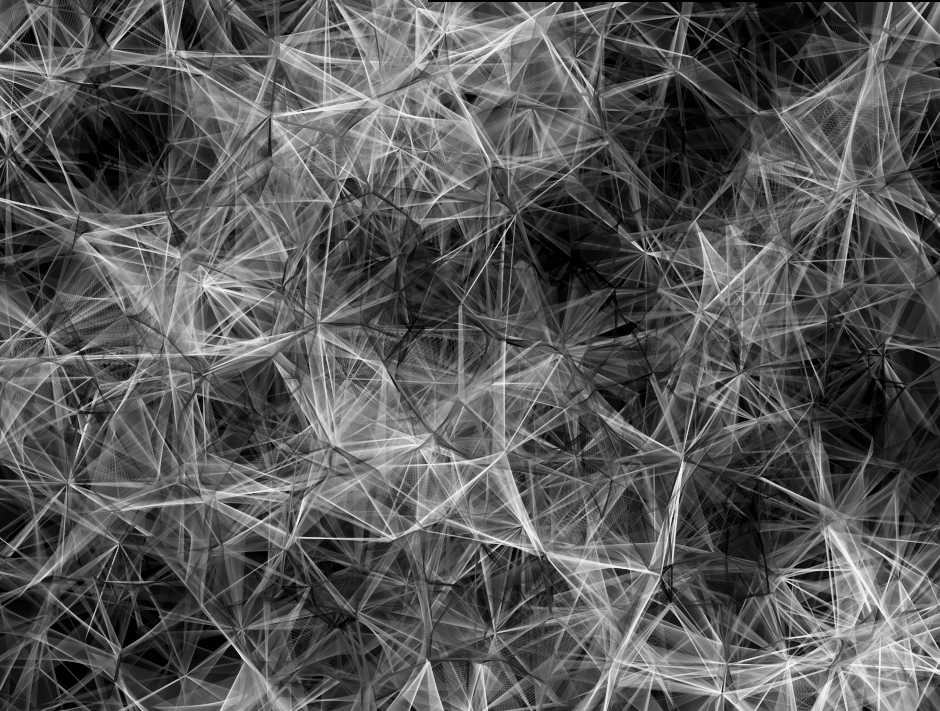
\includegraphics[width=1\paperwidth]{./images/portada.png}}
	\begin{frame}[plain]
		\titlepage
	\end{frame}
}

\section{Estructura del trabajo}

\subsection{Estructura del trabajo}

\begin{frame}
\vspace{-4mm}
\begin{center}
\color{ChetwodeBlue}\large\textbf{Matemáticas:}  
\end{center}
\vspace{-3mm}
\begin{enumerate}
\item \emph{Cyclotomic polynomials at roots of unity}, Bart{\l}omiej Bzd\c{e}ga, Andrés Herrera-Poyatos and Pieter Moree, accepted by Acta Arithmetica, \href{https://arxiv.org/abs/1611.06783}{arXiv:1611.06783}.
\item\emph{ Coefficients and higher order derivatives of cyclotomic polynomials: old and new}, Andrés Herrera-Poyatos and Pieter Moree, \href{https://arxiv.org/abs/1805.05207}{arXiv:1805.05207}.
\item \emph{Isolated factorizations and their applications in simplicial affine semigroups}, Pedro A. García-Sánchez and Andrés Herrera-Poyatos, \href{https://arxiv.org/abs/1804.00885}{arXiv:1804.00885}.
\item \emph{Exponent sequences of cyclotomic numerical semigroups}, Alexandru Ciolan, Pedro A. García-Sánchez, Andrés Herrera-Poyatos and Pieter Moree, on preparation.
\end{enumerate}

\vspace{-5mm}
\begin{center}
\color{ChetwodeBlue}\large\textbf{Informática:}  
\end{center}
\vspace{-3mm}
\begin{enumerate}
\item Algoritmos para detectar polinomios de Kronecker.
\item Herramientas para de visualización de grafos asociados a semigrupos numéricos: \texttt{dot-numericalsgps} and \texttt{FrancyMonoids}.
\end{enumerate}  
\end{frame}

\section{Matemáticas}

\subsection{Semigrupos numéricos}

\begin{frame}
  \begin{definition}[{semigrupo numérico}]
    Un semigrupo numérico $S$ es un submonoide aditivo de $\mathbb{N} = \{0, 1, 2, \ldots\}$ tal que
    $\mathbb{N} \setminus S$ es finito.
  \end{definition}

  \begin{example}
    \centering
    $S = \langle 3,5 \rangle = \{3 a + 5 b : a,b \in \mathbb{N}\} = \{0, 3, 5, 6, 8, \rightarrow\}$
    \begin{table}
      \begin{tabular}{|c|c|c|c|c|c|c|c|c|c|c|c|}
        \hline
        0 & 1 & 2 & 3 & 4 & 5 & 6 & 7 & 8 & 9 & $\cdots$ & $\cdots$ \\
        \hline
        \hline
        1 & 0 & 0 & 1 & 0 & 1 & 1 & 0 & 1 & 1 & $\cdots$ & 1 \\
        \hline
      \end{tabular}
    \end{table}
  \end{example}

  \begin{proposition}
    \begin{itemize}
    \item Todo semigrupo numérico tiene un único sistema de generadores minimal, que es finito. Su cardinal se denomina \textbf{dimensión de inmersión de $S$}.
    \item $S = \left\langle n_1, \ldots, n_e \right\rangle \subseteq \mathbb{N}$ es un semigrupo
      numérico si, y solo si, $\gcd(n_1, \ldots, n_e) = 1$.
    \end{itemize}
  \end{proposition}
\end{frame}

\begin{frame}
  \begin{definition}[{Serie de Hilbert y polinomio del semigrupo}]
    \vspace{2mm}
    \textbf{Serie de Hilbert:}
    \vspace{-8mm}
    \[ \mathrm{H}_S(x) = \sum_{s \in S} x^s = \frac{1}{1-x} - \sum_{g \not \in S} x^{g} \]
    \textbf{Polinomio del \\ semigrupo:}
    \vspace{-10mm}
    \[ \qquad \qquad \mathrm{P}_S(x) = (1-x) \mathrm{H}_S(x) = 1 + (x-1)\sum_{g \not \in S} x^{g} \]
    \vspace{-3mm}
  \end{definition}

  \begin{tcolorbox}[colback=ChetwodeBlue!10,colframe=ChetwodeBlue!60]
    \begin{center}
      {\color{TurkishRose}\textbf{¡Algunas propiedades del semigrupo se caracterizan mediante
          propiedades de $\mathrm{P}_s$}!} \\
      \textbf{Ejemplo:} $S$ es simétrico si, y solo si, $\mathrm{P}_S$ es un palíndromo.
    \end{center}
  \end{tcolorbox}
  
  \begin{example}[$S = \langle 3,5 \rangle = \{0, 3, 5, 6, 8, \rightarrow\}$]
    \vspace*{-7mm}
    \begin{align*}
      \mathrm{H}_S(x) & = \frac{1}{1-x} - x - x^2 -x^4 - x^7 = \frac{1 - x^{15}}{(1-x^3)(1-x^5)} \\
      \mathrm{P}_S(x) & = 1 - x + x^3 - x^4 + x^5 - x^7 + x^8 = \frac{(1-x)(1 - x^{15})}{(1-x^3)(1-x^5)} = \Phi_{15}(x) \\
    \end{align*}  
    \vspace*{-12mm}
  \end{example}
\end{frame}

\subsection{Polinomios ciclotómicos}

\begin{comment}
  \begin{frame}
    \begin{definition}[{polinomios ciclotómicos}]
      Sea $\zeta_n$ una raíz $n$-ésima primitiva de la unidad. El $n$-ésimo polinomio ciclotómico es
      \[ \Phi_n(x)=\prod_{1\le j\le n,~(j,n)=1}(x-\zeta_n^j). \]
    \end{definition}
  
    \begin{itemize}
    \item $\Phi_n$ es el polinomio mínimo de $\zeta_n$ en $\mathbb{Q}$;
    \item $\Phi_n$ es mónico con coeficientes enteros.
    \end{itemize}

  \begin{lemma}[Inversión de M\"obius]
    Sea $n$ un entero positivo con $n \ge 2$. Entonces \vspace*{-1mm}
    \begin{equation*}
      \Phi_n(x) = \prod_{d \, \mid n}(1-x^d)^{\mu(n/d)}.
      \vspace*{-3mm}
    \end{equation*}
  \end{lemma}

  \begin{example}
    \vspace*{-2mm}
    \[ \Phi_{15}(x) = \frac{(1-x)(1 - x^{15})}{(1-x^3)(1-x^5)}\] \vspace*{-2mm}
  \end{example}
\end{frame}
\end{comment}

\begin{frame}
  \begin{definition}[{Polinomios ciclotómicos}]
    Sea $\zeta_n$ una raíz $n$-ésima primitiva de la unidad. El $n$-ésimo polinomio ciclotómico es
    \[ \Phi_n(x)=\prod_{1\le j\le n,~(j,n)=1}(x-\zeta_n^j). \]
  \end{definition}
  
  \begin{itemize}
  \item $\Phi_n$ es el polinomio mínimo de $\zeta_n$ en $\mathbb{Q}$;
  \item $\Phi_n$ es mónico con coeficientes enteros.
  \end{itemize}

  \begin{definition}[{Polinomios de Kronecker}]
    Un polinomio $p \in \mathbb{Z}[x]$ es de Kronecker si todas sus raíces están en el círculo
    unidad, $\{z \in \mathbb{C} : |z| \le 1\}$.
  \end{definition}
  
  \begin{lemma}[Kronecker]
    Un polinomio $p \in \mathbb{Z}[x]$ es de Kronecker si, y solo si, factoriza como producto de un
    monomio y polinomios ciclotómicos.
  \end{lemma}  
\end{frame}

\subsection{Semigrupos numéricos ciclotómicos}

\begin{frame}
  \begin{tcolorbox}[colback=ChetwodeBlue!10,colframe=ChetwodeBlue!60]
    \begin{center}
      \vspace*{-1mm}
      {\color{TurkishRose}\textbf{Cyclotomic numerical semigroups}} \\
      A. Ciolan, P.A. García-Sánchez, and P. Moree \\
      SIAM J. Discrete Math. 30 (2016).
    \end{center}
    \vspace*{-6mm}
  \end{tcolorbox}

  \begin{definition}[{Semigrupos numéricos ciclotómicos}]
    Un semigrupo numérico $S$ es ciclotómico si su polinomio es de Kronecker.
  \end{definition}

  \begin{definition}[{Intersecciones completas}]
    Un semigrupo numérico $S$ es intersección completa si todas sus presentaciones minimales tienen $\mathem{e}(S)-1$ relaciones.
  \end{definition}

  \begin{theorem} [Ciolan, García-Sánchez, Moree]
    Sea $S$ un semigrupo numérico.
    \begin{enumerate}
    \item Si $S$ es intersección completa, entonces $S$ es ciclotómico.
    \item Si $S$ es ciclotómico, entonces es simétrico.
    \end{enumerate}
  \end{theorem}
\end{frame}

\begin{frame}
  \begin{tcolorbox}[colback=ChetwodeBlue!10,colframe=ChetwodeBlue!60]
    \begin{center}
      \vspace*{-1mm}
      {\color{TurkishRose}\textbf{Cyclotomic numerical semigroups}} \\
      A. Ciolan, P.A. García-Sánchez, and P. Moree \\
      SIAM J. Discrete Math. 30 (2016).
    \end{center}
    \vspace*{-6mm}
  \end{tcolorbox}

  \begin{definition}[{Semigrupos numéricos ciclotómicos}]
    Un semigrupo numérico $S$ es ciclotómico si su polinomio es de Kronecker.
  \end{definition}

  \begin{theorem} [Ciolan, García-Sánchez, Moree]
    Sea $S$ un semigrupo numérico.
    \begin{enumerate}
    \item Si $S$ es intersección completa, entonces $S$ es ciclotómico.
    \item Si $S$ es ciclotómico, entonces es simétrico.
    \end{enumerate}
  \end{theorem}

  \begin{conjecture}
    \vspace*{-1mm}
    \begin{enumerate}
    \item Un semigrupo numérico es ciclotómico si, y solo si, es intersección completa.
    \item Para cada $k \ge 4$ existe un semigrupo numérico $S_k$ simétrico con dimensión de inmersión $k$ que no es ciclotómico.
    \end{enumerate}
    \vspace*{-1mm}
  \end{conjecture}
\end{frame}

\subsection{Cyclotomic polynomials at roots of unity}

\begin{frame}
  \begin{tcolorbox}[colback=ChetwodeBlue!10,colframe=ChetwodeBlue!60]
    \begin{center}
      \vspace*{-1mm} {
        \color{TurkishRose}\textbf{Cyclotomic polynomials at roots of unity}} \\
      Bart{\l}omiej Bzd\c{e}ga, Andr\'es Herrera-Poyatos and Pieter Moree\\
      Acta Arithmetica (2018), \href{https://arxiv.org/abs/1611.06783}{arXiv:1611.06783}
    \end{center}
    \vspace*{-6mm}
  \end{tcolorbox}

  \begin{problem}
    Evaluar $\Phi_n$ en las raíces de la unidad.
  \end{problem}

  \begin{lemma}[Evaluación en 1]
    \vspace*{-3mm}
    \[ \Phi_n(1) = \begin{cases} 0 & \hbox{si } n=1;\\
        p & \hbox{si } n=p^k \hbox{ para algún primo } p;\\
        1 & \hbox{en caso contrario.}
      \end{cases} \] \vspace*{-4mm}
  \end{lemma}
  \vspace*{-1mm}
  \begin{lemma}[Evaluación en -1]
    \vspace*{-3mm}
    \[ \Phi_n(-1) = \begin{cases} -2 & \hbox{si } n=1;\\
        0 & \hbox{si } n=2;\\
        p & \hbox{si } n=2p^k \hbox{ para algún primo } p;\\
        1 & \hbox{en caso contrario.}
      \end{cases} \] \vspace*{-4mm}
  \end{lemma}
\end{frame}

\begin{frame}
  \begin{tcolorbox}[colback=ChetwodeBlue!10,colframe=ChetwodeBlue!60]
    \begin{center}
      \vspace*{-1mm} {
        \color{TurkishRose}\textbf{Cyclotomic polynomials at roots of unity}} \\
      Bart{\l}omiej Bzd\c{e}ga, Andr\'es Herrera-Poyatos and Pieter Moree\\
      Acta Arithmetica (2018), \href{https://arxiv.org/abs/1611.06783}{arXiv:1611.06783}
    \end{center}
    \vspace*{-6mm}
  \end{tcolorbox}

  \begin{theorem}[Evaluación de $\Phi_n$ en raíces de la unidad]
    Sean $n,m > 1$ enteros coprimos y $\xi_m$ una raíz $m$-ésima primitiva de la unidad. Entonces
    \vspace*{-3mm}
    \begin{equation*}
      \Phi_n(\xi_m) =
      \exp\left(\sum_{\chi\in\widehat{\mathbb{Z}_m^{\times}}} \hat{f}(\chi)\chi(n)\prod_{p\mid
          n}(1-\overline{\chi}(p))\right),
    \end{equation*}
    donde $f(k) = \log(1 - \xi_m^k)$.
  \end{theorem}

  \begin{theorem}[Originalmente demostrado por Vaughan, 1975]
    Existen infinitos enteros positivos $n$ tales que \vspace{-2mm}
    \[ \log\log H(\Phi_n) > \log(2) \frac{\log n}{\log\log n}. \] \vspace{-4mm}
  \end{theorem}
\end{frame}

\begin{frame}
  \vspace*{-1mm}
  \begin{example}[$n = 3234846615 = 3 \cdot 5 \cdot 7 \cdot 11 \cdot 13 \cdot 17 \cdot 19 \cdot 23
    \cdot 29$]
    \vspace*{-3mm}
    \begin{center}
      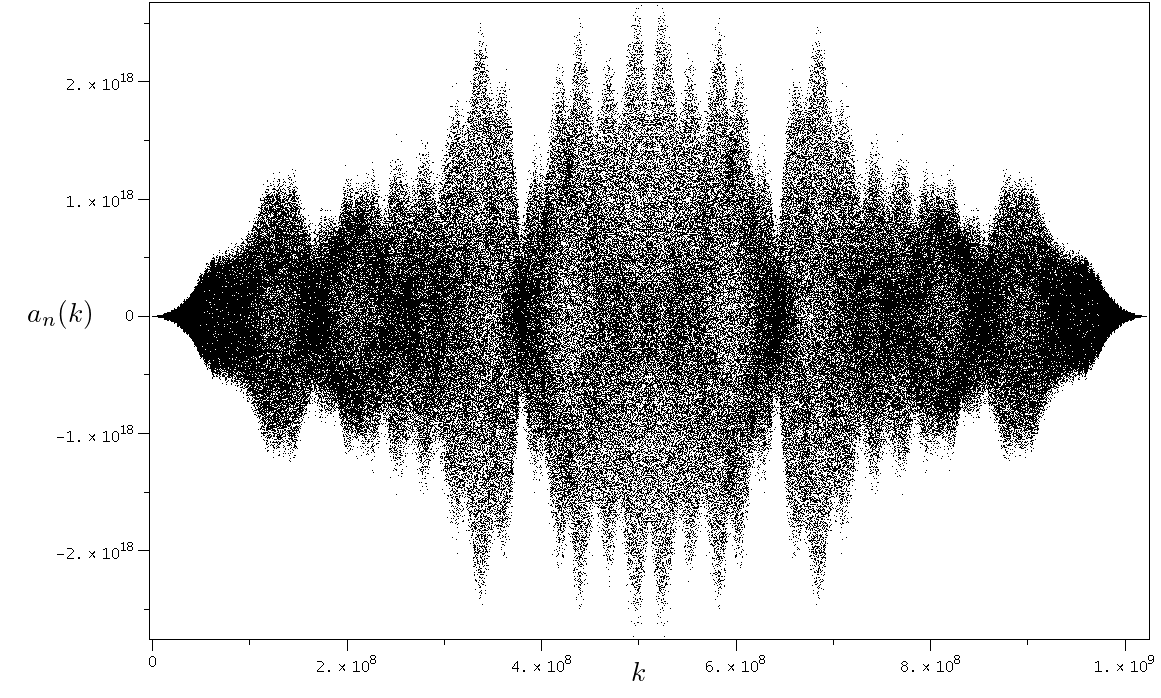
\includegraphics[width=\textwidth]{./images/cyclo-coeffs.png}
    \end{center}
    \vspace*{-4mm}
  \end{example}
  \vspace*{-1mm}
  \begin{tcolorbox}[colback=ChetwodeBlue!10,colframe=ChetwodeBlue!60]
    \begin{center}
      \vspace*{-2mm} {\color{TurkishRose}\textbf{Si el número de factores primos distintos de $n$ es
          grande aparecen patrones complejos que no sabemos explicar.}}
    \end{center}
    \vspace*{-5mm}
  \end{tcolorbox}
\end{frame}

\begin{comment}
  \begin{frame}
    \begin{columns}
      \column{0.5\textwidth}
      \begin{lemma}[Evaluación de $\Phi_n(i)$]
        \begin{center}
          \begin{tabular}{|c|c|}
            \hline
            $ n $ & $ \Phi_n(i) $  \\
            \hline
            $1$ & $i-1$  \\
            \hline
            $2$ & $i+1$  \\
            \hline
            $4$ & $0$  \\
            \hline
            $ 4p^k $ & $ p $\\
            \hline
            $ p_3^k $ & $ (-1)^{k+1}i $\\
            \hline
            $ 2p_3^k $ & $ (-1)^k i $\\
            \hline
            $ p_3^kq_3^l, ~2p_3^kq_3^l $ & $ -1 $\\
            \hline
            En otro caso & 1 \\
            \hline
          \end{tabular}
        \end{center}
        donde $ p,p_3$ y $q_3 $ son primos tales que $p_3\ne q_3$ y
        $ p_3\equiv q_3\equiv 3\pmod 4 $.
      \end{lemma}
      \begin{tcolorbox}[colback=ChetwodeBlue!10,colframe=ChetwodeBlue!60]
        \begin{center} {\color{TurkishRose}\textbf{Con mucha paciencia y cuidado podemos calcular
              éstas y más tablas.}}
        \end{center}
        \vspace*{-4mm}
      \end{tcolorbox}

      \column{0.5\textwidth}
      \begin{lemma}[Evaluación de $\Phi_n(\zeta_3)$]
        
        \begin{center}
          \begin{tabular}{|c|c|}
            \hline
            $ n $ & $ \Phi_n(\zeta_3) $  \\
            \hline
            $1$ & $\zeta_3-1$  \\
            \hline
            $3$ & $0$  \\
            \hline
            $3 p^{k}$ & $p$  \\
            \hline
            $ q^{k} $ & $ -1/\zeta$\\
            \hline
            $ 3q^{k} $ & $ -q\zeta$\\
            \hline
            $ q_1^{e_1} \ldots q_r^{e_r},~r\ge 2$ & $ 1/{\zeta} $\\
            \hline
            $ 3q_1^{e_1} \ldots q_r^{e_r},~r\ge 2 $ & $\zeta$\\
            \hline
            En otro caso & 1 \\
            \hline
          \end{tabular}
        \end{center}
        \fontsize{9}{5}\selectfont
        \begin{enumerate}
        \item $p\not\equiv 2 \pmod{3}$ es primo;
        \item $q \equiv 2 \pmod{3}$ es primo;
        \item $q_1, \ldots, q_r$ son primos distintos congruentes con $2$ módulo $3$ con $r\ge 2$;
        \item $\zeta=(\zeta_3)^{\wedge} (-1)^{\Omega(n)-\omega(n)}$.
        \end{enumerate}
      \end{lemma}
    \end{columns}
  \end{frame}
\end{comment}

\subsection{Coefficients and higher order derivatives of cyclotomic polynomials: old and new}

\begin{frame}
  \begin{tcolorbox}[colback=ChetwodeBlue!10,colframe=ChetwodeBlue!60]
    \begin{center}
      \vspace*{-1mm} {
        \color{TurkishRose}\textbf{Coefficients and higher order derivatives of cyclotomic polynomials: old and new}} \\
      Andr\'es Herrera-Poyatos and Pieter Moree \\
      \href{https://arxiv.org/abs/1805.05207}{arXiv:1805.05207}
    \end{center}
    \vspace*{-4mm}
  \end{tcolorbox}

  \begin{theorem}[Lehmer, 1966]
    Sean $k \ge 1$ y $n\ge 2$ enteros. Entonces
    \[(\log \Phi_n)^{(k)}(1) = \sum_{j=1}^{k} \frac{B_j^+ s(k,j)}{j} J_j(n).\]
  \end{theorem}

  \begin{theorem} 
    \[\frac{\Phi_n^{(k)}(1)}{\Phi_n(1)}= \mathcal{B}_k\Big(\sum_{j=1}^{1} \frac{B_j^+ s(1,j)}{j}
      J_j(n), \dots, \sum_{j=1}^{k} \frac{B_j^+ s(k,j)}{j} J_j(n)\Big).\]
  \end{theorem}
\end{frame}

\begin{frame}
  \begin{tcolorbox}[colback=ChetwodeBlue!10,colframe=ChetwodeBlue!60]
    \begin{center}
      \vspace*{-1mm} {
        \color{TurkishRose}\textbf{Coefficients and higher order derivatives of cyclotomic polynomials: old and new}} \\
      Andr\'es Herrera-Poyatos and Pieter Moree \\
      \href{https://arxiv.org/abs/1805.05207}{arXiv:1805.05207}
    \end{center}
    \vspace*{-4mm}
  \end{tcolorbox}

  \begin{theorem} 
   Sea $f$ un polinomio de Kronecker con $f(0) \ne 0$ y $f(1) \ne 0$. Escribimos $f = \prod_{\mathcal{D}} \Phi_d^{e_d}$. Para cada entero
    $k\ge 2$ se tiene
    \[ \sum_{j = 1}^k \stirlingtwo{k}{j} (\log f)^{(j)}(1) = \frac{B_{k}^+}{k} \sum_{d \in
        \mathcal{D}} e_d J_k(d). \] \vspace*{-4mm}
  \end{theorem}

  \begin{theorem} 
    Para cada $k \ge 4$ el semigrupo numérico
    \[S_k = \{0, k, k+1, k+2, \rightarrow\} \setminus \{2k-1\}\]
    es simétrico, tiene dimensión de inmersión $k$ y no es ciclotómico.    
  \end{theorem}
\end{frame}

\subsection{Isolated factorizations and their applications in simplicial affine semigroups}

\begin{frame}
  \begin{tcolorbox}[colback=ChetwodeBlue!10,colframe=ChetwodeBlue!60]
    \begin{center}
      \vspace*{-1mm} {\color{TurkishRose}\textbf{Isolated factorizations and their applications in
          simplicial affine
          semigroups}} \\
      Pedro A. Garc\'ia-Sánchez and Andrés Herrera-Poyatos \\
      \href{https://arxiv.org/abs/arXiv:1804.00885}{arXiv:1804.00885}
    \end{center}
    \vspace*{-4mm}
  \end{tcolorbox}

  Sea $S$ un semigrupo numérico y $A = \{n_1, \ldots, n_e\}$ un sistema de generadores minimal de
  $A$. Definimos $\varphi \colon \mathbb{N}^e \to S$ como
  $\varphi(x_1, \ldots, x_e) = x_1 n_1 + \cdots + x_e n_e$.
  
  \begin{definition}[factorizaciones aisladas]
    \begin{itemize}
    \item Las factorizaciones de $s \in S$ son los elementos de $\mathrm{Z}(s) = \varphi^{-1}(s)$.
    \item $x \in \mathrm{Z}(s)$ es aislada si $\left\langle x, y \right\rangle = 0$ para todo
      $y \in \mathbb{Z}(s) \setminus \{x\}$.
    \end{itemize}
  \end{definition}

  \textbf{Aplicación:} Análisis de nuevas familias de semigrupos numéricos
    \vspace*{-4mm}
  
  \begin{gather*}
    \text{Único elemento de Betti} \subset {\color{TurkishRose}\text{Betti divisible}} \subset {\color{TurkishRose}\text{Betti ordenado}} \\
    \subset {\color{TurkishRose}\text{Intersección completa con solo un elemento Betti minimal}} \\
    \subset \alpha\text{-rectangular} \subset \text{Libre} \subset \text{Intersección completa}.
  \end{gather*}
\end{frame}
  
\subsection{Exponent sequences of cyclotomic numerical semigroups}

\begin{frame}
  \begin{tcolorbox}[colback=ChetwodeBlue!10,colframe=ChetwodeBlue!60]
    \begin{center}
      \vspace*{-1mm} {\color{TurkishRose}\textbf{Exponent sequences of cyclotomic numerical semigroups}} \\
      Alexandru Ciolan, Pedro A. Garc\'ia-Sánchez, Andrés Herrera-Poyatos and Pieter Moree
    \end{center}
    \vspace*{-4mm}
  \end{tcolorbox}

  
  \begin{definition}[Secuencia de exponentes ciclotómicos]
    Sea $S$ un semigrupo numérico ciclotómico. Existe una secuencia $\{f_d\}$ con soporte finito tal
    que \vspace*{-3mm}
    \[ \mathrm{P}_S(x) = \prod_{d = 1}^{\infty} (1 - x^d)^{f_d}, \] Esta secuencia se denomina
    secuencia de exponentes ciclotómicos de $S$.
    
    \begin{enumerate}
    \item $\Omega_+ = \{d \in \mathbb{N}: f_d > 0\}$;
    \item $\Omega_- = \{d \in \mathbb{N}: f_d < 0\}$.
    \end{enumerate}
  \end{definition}

  \begin{theorem}
    $\Omega_-$ es un sistema de generadores de $S$ y $\Omega_+ \setminus \{1\} \subset S$.
  \end{theorem}
\end{frame}

\begin{frame}
  \begin{tcolorbox}[colback=ChetwodeBlue!10,colframe=ChetwodeBlue!60]
    \begin{center}
      \vspace*{-1mm} {\color{TurkishRose}\textbf{Exponent sequences of cyclotomic numerical semigroups}} \\
      Alexandru Ciolan, Pedro A. Garc\'ia-Sánchez, Andrés Herrera-Poyatos and Pieter Moree
    \end{center}
    \vspace*{-4mm}
  \end{tcolorbox}

  \begin{theorem} 
    $\Lambda \subseteq \Omega \setminus (A \cup \{1\})$ con:
    \begin{enumerate}
    \item $\Lambda$ está totalmente ordenado con respecto a $\le_S$, el orden del semigrupo;
    \item si $\alpha \in \Lambda$ y $s \in \Omega \setminus (A \cup \{1\})$ con $s \le_S \alpha$,
      entonces $s \in \Lambda$.
    \end{enumerate}
    Entonces $\Lambda \subseteq \mathrm{Betti}(S) \cap \Omega_+$.
  \end{theorem}

  \begin{theorem}
    Sea $A$ un sistema de generadores minimal de $S$.
    \begin{enumerate}
    \item $S$ es Betti ordenado si, y solo si, $S$ es ciclotómico y $\Omega^* \setminus (A \cup \{1\})$ está totalmente
      ordenado con respecto a $\le_S$.
    \item $S$ es Betti divisible si, y solo si, $S$ es ciclotómico y $\Omega^{*} \setminus (A \cup \{1\})$ está totalmente
      ordenado con respecto a la divisibilidad de enteros.
    \end{enumerate}
  \end{theorem}  
\end{frame}

\section{Informática}

\subsection{Algoritmos para detectar polinomios de Kronecker}

\begin{frame}
  \begin{center}
  {\color{ChetwodeBlue}\Large\textbf{Algoritmos para detectar polinomios de Kronecker}}    
  \end{center}

\begin{tcolorbox}[colback=ChetwodeBlue!10,colframe=ChetwodeBlue!60]
\begin{itemize}
\item \textbf{Estudio del estado del arte.}
\item \textbf{Desarrollo de nuevas propuestas.}
\end{itemize}
  {\color{TurkishRose} \textbf{Aplicaciones:}}
  \begin{enumerate}
\item Detección de semigrupos numéricos ciclotómicos.
\item Detección de semigrupos numéricos intersecciones completas \\
      (si $\text{ciclotómico} = \text{intersección completa}$).
\end{enumerate}
  \end{tcolorbox}

  \begin{columns}
  \column{0.2\textwidth}
  
\includegraphics[width=\textwidth]{./images/github.png}
  \column{0.7\textwidth}
  
  \begin{itemize}
  \item Implementación en GAP.
  \item Licencia GPLv2.
  \item El mejor algoritmo se ha añadido al paquete \texttt{numericalsgps} de GAP. \\ \url{gap-packages.github.io/numericalsgps/}
  \end{itemize}
  \end{columns}

\end{frame}

\begin{frame}{Algoritmos para detectar polinomios de Kronecker}
  
  \begin{enumerate}
  \item \textbf{Algoritmo propuesto por Pieter Moree.}
    \begin{itemize}
    \item Basado en nuestro trabajo sobre polinomios de Kronecker.
    \item Complejidad: $O((\deg p)^6)$ en el peor caso.
    \end{itemize}
  \item \textbf{Algoritmo propuesto por David Boyd.}
    \begin{itemize}
    \item Basado en secuencias de Sturm.
    \item Complejidad: $\theta((\deg p)^3)$.
    \end{itemize}
  \item \textbf{Algoritmo propuesto por Bradford and Davenport.}
    \begin{itemize}
    \item Basado en el método de Graeffe.
    \item Complejidad: Difícil de analizar teóricamente. \\ \qquad \qquad \quad \ \ $O((\deg p)^4)$ en el peor caso.
    \end{itemize}
  \item {\textbf{\color{TurkishRose}Nueva propuesta basada en el algoritmo de Bradford y
        Davenport.}}
    \begin{itemize}
    \item Complejidad: $O((\deg p)^3)$ en el peor caso.
    \item Es el mejor tanto en la teoría como en la práctica.
    \end{itemize}
  \end{enumerate}

  {\color{ChetwodeBlue}\textbf{Para medir la complejidad, suponemos que los coeficientes están acotados.}}
  \end{frame}

  \begin{frame}
    \begin{figure}[H]
      \centering
      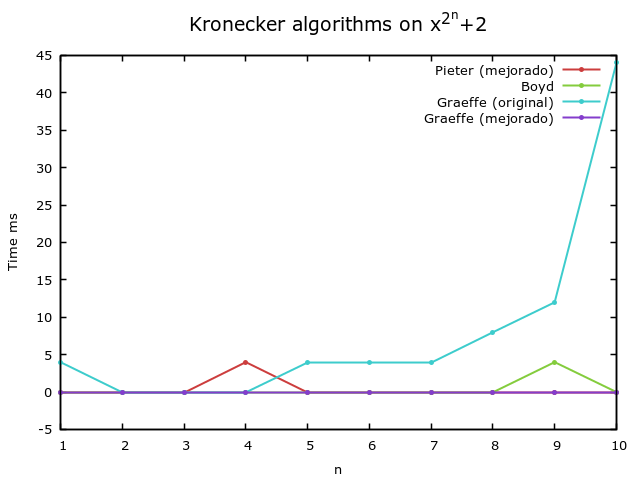
\includegraphics[width=\textwidth]{./images/fast_4.png}      
    \end{figure}
  \end{frame}

  \begin{frame}
    \begin{figure}[H]
      \centering
      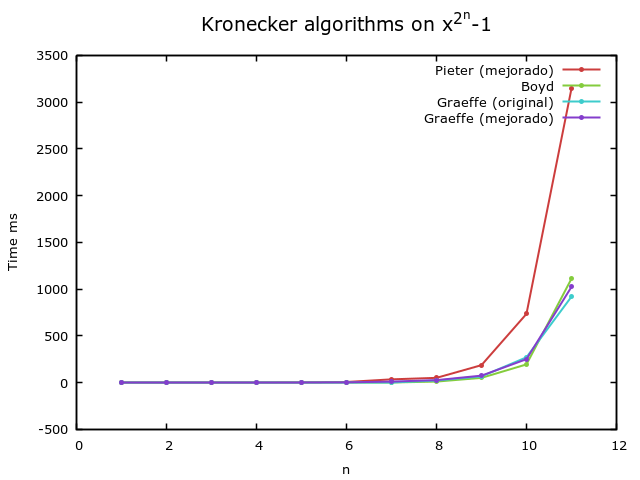
\includegraphics[width=\textwidth]{./images/fast_1.png}      
    \end{figure}
  \end{frame}

  \begin{frame}
    \begin{figure}[H]
      \centering
      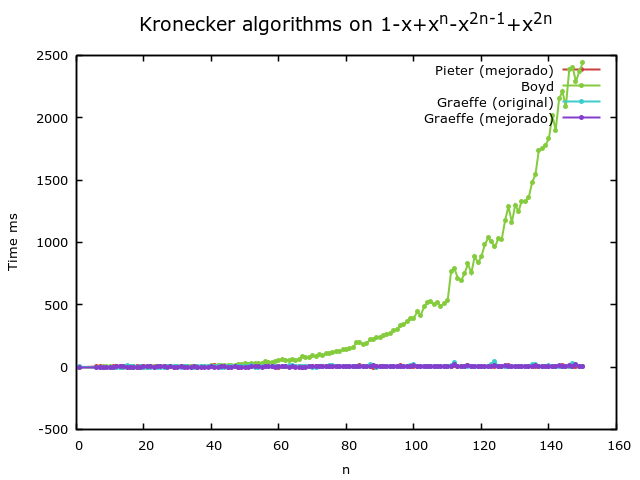
\includegraphics[width=\textwidth]{./images/fast_pedro.png}      
    \end{figure}
  \end{frame}

  \subsection{Herramientas de visualización para semigrupos numéricos}

\begin{frame}
  \begin{center}
  {\color{ChetwodeBlue}\Large\textbf{Herramientas de visualización para semigrupos numéricos}}    
  \end{center}

  \begin{tcolorbox}[colback=ChetwodeBlue!10,colframe=ChetwodeBlue!60]
\textbf{Motivación: } visualizar grafos asociados a semigrupos numéricos
  \end{tcolorbox}
  
\begin{enumerate}
\item \textbf{dot-numericalsgps}  
\begin{itemize}
\item Genera código DOT
\item El código DOT se visualiza mediante \texttt{graphviz} o similar
\item Se ha añadido a la última versión de \texttt{numericalsgps}:
  \url{gap-packages.github.io/numericalsgps/doc/chap14.html}
\end{itemize}
\item \textbf{FrancyMonoids}
\begin{itemize}
\item Genera diagramas interactivos de \texttt{3djs}
\item Utiliza el paquete de GAP \texttt{Francy}:
  \url{https://github.com/mcmartins/francy}
\item Se encuentra en la organización de paquetes de GAP en GitHub:
  \url{https://gap-packages.github.io/FrancyMonoids/}
\end{itemize}
\end{enumerate}

  \begin{tcolorbox}[colback=ChetwodeBlue!10,colframe=ChetwodeBlue!60]
\begin{itemize}
\item Ambos paquetes se pueden usar con jupyter
\item Tienen licencia GPLv2
\end{itemize}
  \end{tcolorbox}
\end{frame}
  
\begin{frame}[fragile]
  \begin{center}
  {\color{ChetwodeBlue}\Large\textbf{dot-numericalsgps}}    
  \end{center}
\begin{minted}[bgcolor=backg]{c}
LoadPackage("numericalsgps");
S := NumericalSemigroup(4,6,9);
DotSplash(DotTreeOfGluingsOfNumericalSemigroup(S, 4));
\end{minted}

\begin{center}
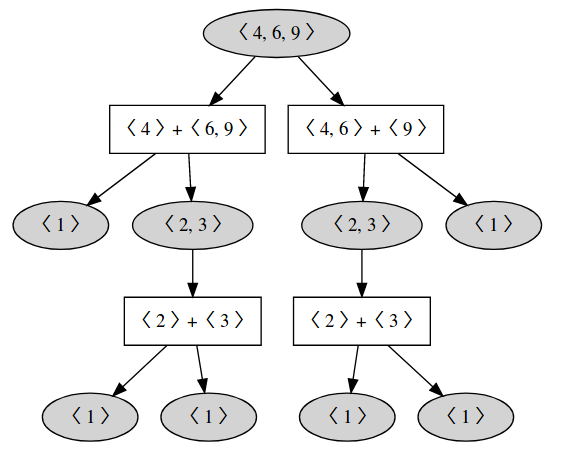
\includegraphics[width=0.6\textwidth]{./images/tree-gluings.png}  
\end{center}
\end{frame}

\begin{frame}[fragile]
  \begin{center}
  {\color{ChetwodeBlue}\Large\textbf{dot-numericalsgps}}    
  \end{center}
\begin{minted}[bgcolor=backg]{c}
LoadPackage("numericalsgps");
S := NumericalSemigroup(4,6,9);
f:=FactorizationsElementWRTNumericalSemigroup(30,S);
JupyterSplashDot(DotFactorizationGraph(f));
\end{minted}

\begin{center}
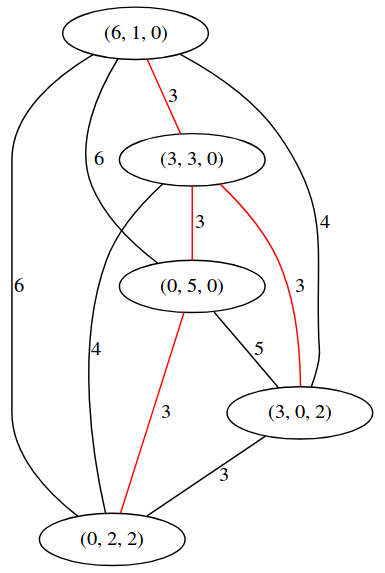
\includegraphics[width=0.36\textwidth]{./images/factorizations.png}  
\end{center}
\end{frame}

\begin{frame}[fragile]
  \begin{center}
  {\color{ChetwodeBlue}\Large\textbf{dot-numericalsgps}}    
  \end{center}
\begin{minted}[bgcolor=backg]{c}
LoadPackage("numericalsgps");
S := NumericalSemigroup(4,6,9);
JupyterSplashDot(DotOverSemigroupsNumericalSemigroup(S));
\end{minted}

\begin{center}
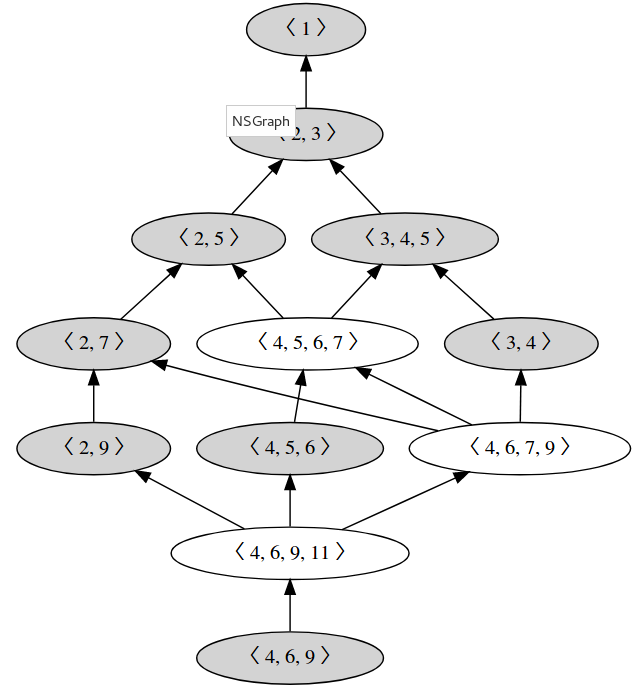
\includegraphics[width=0.53\textwidth]{./images/over-semigroups.png}  
\end{center}
\end{frame}

\begin{frame}[fragile]
  \begin{center}
  {\color{ChetwodeBlue}\Large\textbf{FrancyMonoids}}    
  \end{center}
\begin{minted}[bgcolor=backg]{c}
LoadPackage("numericalsgps");
LoadPackage("FrancyMonoids");
s:=NumericalSemigroup(5,7,9,11);
DrawHasseDiagramOfNumericalSemigroup(s,AperyList(s,10));
\end{minted}

\begin{center}
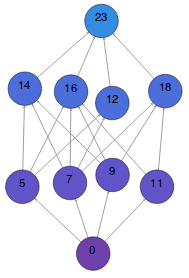
\includegraphics[width=0.35\textwidth]{./images/apery.png}  
\end{center}
\end{frame}

\begin{frame}[fragile]
  \begin{center}
  {\color{ChetwodeBlue}\Large\textbf{FrancyMonoids}}    
  \end{center}
\begin{minted}[bgcolor=backg]{c}
LoadPackage("numericalsgps");
LoadPackage("FrancyMonoids");
s:=NumericalSemigroup(20,21,22,23,24,25,26,27,28);
DrawRosalesGraph(67,s);
\end{minted}

\begin{center}
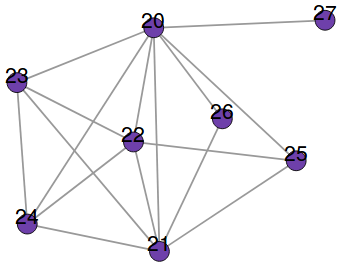
\includegraphics[width=0.6\textwidth]{./images/rosales.png}  
\end{center}
\end{frame}

\begin{frame}[fragile]
  \begin{center}
  {\color{ChetwodeBlue}\Large\textbf{FrancyMonoids}}    
  \end{center}
\begin{minted}[bgcolor=backg]{c}
LoadPackage("numericalsgps");
LoadPackage("FrancyMonoids");
s:=NumericalSemigroup(3,4,5);
gens:=s->Difference(MinimalGenerators(s), 
                    [Multiplicity(s)]);
DrawTreeOfSonsOfNumericalSemigroup(s,5,gens);
\end{minted}

\begin{center}
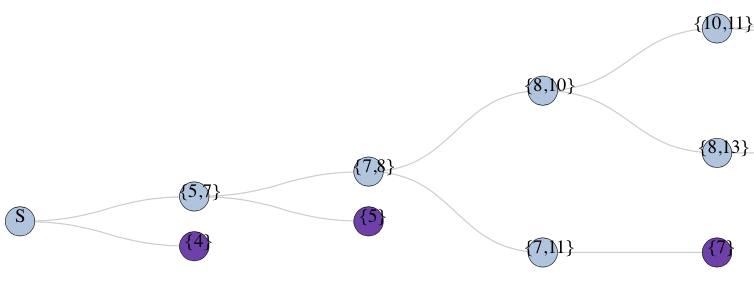
\includegraphics[width=\textwidth]{./images/tree-semigroups.png}  
\end{center}
\end{frame}

\section{Trabajo futuro}

\subsection{Trabajo futuro}

\begin{frame}
  \begin{center}
    {\color{ChetwodeBlue}\Large\textbf{Trabajo en proceso}}
  \end{center}
  \vspace{-3mm}
  \begin{enumerate}
  \item \textbf{Secuencias de exponentes ciclotómicos}
    \begin{itemize}
    \item Eliminar la hipótesis de que $S$ sea ciclotómico en los resultados acerca de $\Omega_-$ y
      $\Omega_+$.
    \item Aplicación a semigrupos numéricos ciclotómicos con altura y profundidad fija.
    \item Estudio de la longitud de un semigrupo numérico ciclotómico.
    \end{itemize}
  \item \textbf{Semigrupos simpliciales afines:}
    \begin{itemize}
    \item Generalizar el concepto de semigrupo numérico $\beta$-rectangular y $\gamma$-rectangular.
    \item Estudio de los semigrupos $c^{*}$-rectangulare, $\bar{c}$-rectangulares y
      $c$-rectangulares.
    \end{itemize}
  \item \textbf{Semigrupos numéricos intersecciones completas:}
    \begin{itemize}
    \item Nuevas caracterizaciones en terminos de $\mathrm{Betti}(S)$.
    \end{itemize}
  \item \textbf{Algoritmos para detectar polinomios de Kronecker:}
    \begin{itemize}
    \item Publicar nuestro estudio y nuestras propuestas.
    \end{itemize}
  \item \textbf{Librerías \texttt{numericalsgps-dot} y \texttt{FrancyMonoids}:}    
    \begin{itemize}
    \item Desarrollo de nuevas funciones.
    \end{itemize}
  \end{enumerate}
\end{frame}

{ \usebackgroundtemplate{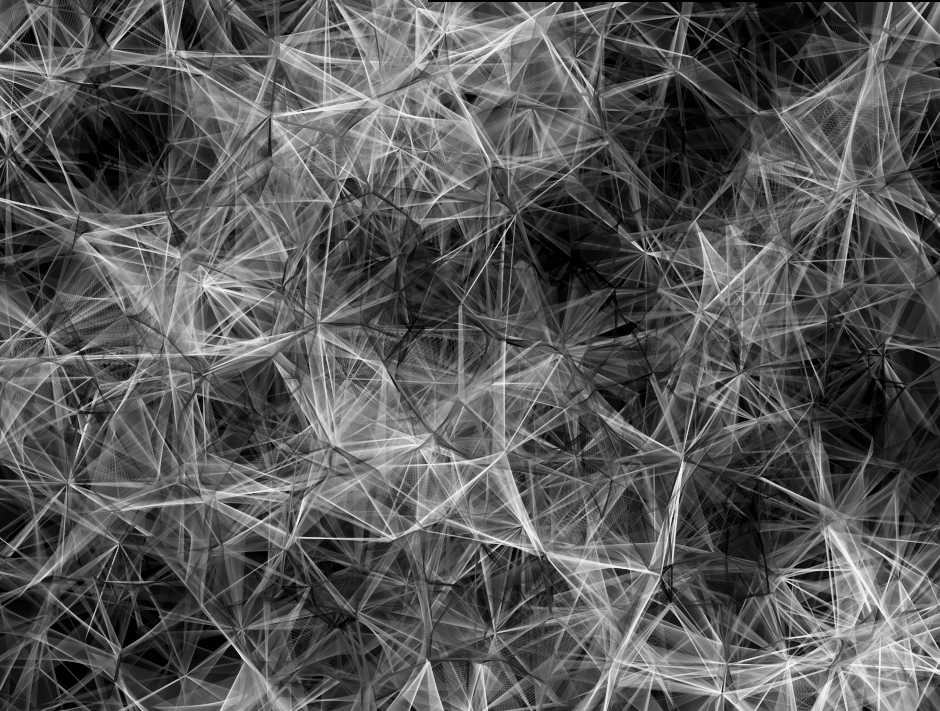
\includegraphics[width=1\paperwidth]{./images/portada.png}}
  \begin{frame}[plain]
    \vspace{0.1\paperheight}
    \begin{titleBox}
      \begin{beamercolorbox}[sep=8pt,center]{title}
        \usebeamerfont{title}\textbf{¡Gracias por su atención!}
      \end{beamercolorbox}

	\begin{beamercolorbox}[sep=8pt,center]{author}	
          \usebeamerfont{author}\large\textbf{\docauthor} \\
          \usebeamerfont{title}\large\docemail
        \end{beamercolorbox}
      \end{titleBox}
    \end{frame}
  }

\end{document}
